\documentclass{article}
\usepackage{graphicx}
\usepackage{listings}

\lstset{
	language=C,
	basicstyle=\footnotesize,
	numbers=left,
	stepnumber=1,
	showstringspaces=false,
	tabsize=1,
	breaklines=true,
	breakatwhitespace=false,
}

\def \unidad{Universidad Tecnológica de Tijuana}
\def \programa{Ingeniería En Desarrollo Y Gestión De Software}
\def \curso{Aplicaciones Web Progresivas}
\def \titulo{Mockups}

\def \autores{
	Garcia Gonzales Christian Andres\\
	Lopez Bautista Cristian Alexis\\
	Mercado Juarez Angel Hayr\\
	Salas Diaz Guillermo\\
	Santillan Galaviz Ken Antonio\\
	
	\vspace{0.5cm}
	
	Teacher \\
	Dr. Ray Brunett Parra
}
\def \fecha{02 February 2024}
\def \lugar{Tijuana B.C, México}

\begin{document}
	\begin{titlepage}
    \begin{center}
        \vspace*{1cm}
        
        
\includegraphics[width=0.8\linewidth]{images/logo_utt.jpeg}\\
        \LARGE
        \unidad\\
        \programa\\
        \curso
        
        \vspace{1cm}
        
        \Huge
        \textbf{\titulo}
            
        \vspace{0.5cm}
        \LARGE
            
        \vspace{0.5cm}
        \large    
         \autores
            
        \vfill
        
        \lugar\\
        \fecha
        
    \end{center}
\end{titlepage}
	
	\newpage
	\tableofcontents
	
	\newpage
	\section{Introduction}
	In the realm of security services within a company, the implementation of Progressive Web Apps (PWAs) becomes not only relevant but crucial. Our proposed application serves the specific purpose of facilitating rapid security consultations within an organization. The emphasis lies in the quick retrieval of information from an individual's uniform through the scanning of QR codes.
	

	\section{Adaptability to Mobile Devices}
	\begin{figure}[h]
		\centering
		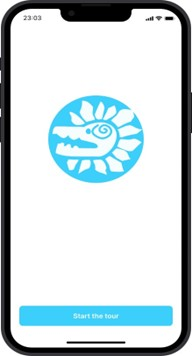
\includegraphics[width=0.2\linewidth]{images/1.jpg}
		\hspace{0.05\linewidth}
		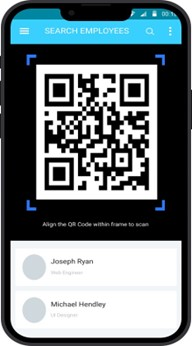
\includegraphics[width=0.2\linewidth]{images/2.jpg}
		\hspace{0.05\linewidth}
		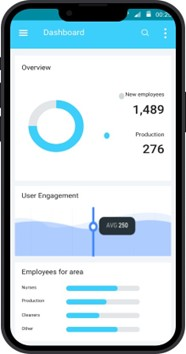
\includegraphics[width=0.2\linewidth]{images/3.jpg}
	\end{figure}
	
	Given the dynamic nature of security operations, personnel often need to access critical information on the go. The adaptability of our PWA to various mobile devices ensures that security consultations can be conducted seamlessly on smartphones and tablets, providing flexibility and efficiency in daily tasks.
	

	\section{Enhanced Offline Experience}
	\begin{figure}[h]
		\centering
		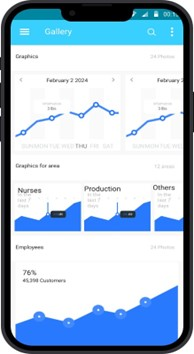
\includegraphics[width=0.2\linewidth]{images/4.jpg}
		\hspace{0.05\linewidth}
		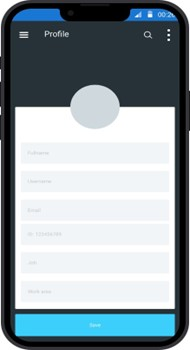
\includegraphics[width=0.2\linewidth]{images/5.jpg}
		\hspace{0.05\linewidth}
		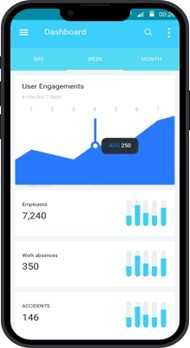
\includegraphics[width=0.2\linewidth]{images/6.jpg}
	\end{figure}
	
	Security situations can arise in areas with limited or no network connectivity. The enhanced offline experience provided by our PWA ensures that critical information remains accessible even in such circumstances. This is vital for immediate response and decision-making during emergencies.
	

	\section{Quick Implementation and Updates}
	\begin{figure}[h]
		\centering
		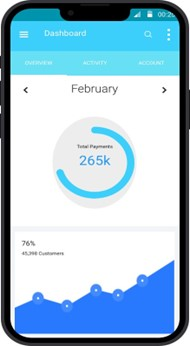
\includegraphics[width=0.2\linewidth]{images/7.jpg}
		\hspace{0.05\linewidth}
		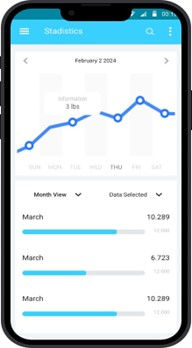
\includegraphics[width=0.2\linewidth]{images/8.jpg}
		\hspace{0.05\linewidth}
		% Add a description for the last image
	\end{figure}
	
	The rapid deployment of security applications is paramount. Our PWA allows for quick implementation and updates without the need for lengthy approval processes. This ensures that the application can promptly adapt to changing security protocols, incorporate bug fixes, and introduce new features as needed.
	

	\section{Efficient QR Code Scanning}
	\begin{flushleft}
		A distinctive feature of our application is its ability to efficiently scan QR codes from the uniforms of individuals. This streamlined process accelerates the retrieval of pertinent information about an accident or incident, facilitating a rapid and informed response from security personnel.
	\end{flushleft}
	
	\newpage
	\section{Conclusion}
	In conclusion, the implementation of Progressive Web Apps (PWAs) for our quick security consultation application is a strategic decision. It not only ensures adaptability to various mobile devices and an enhanced offline experience but also enables rapid implementation and updates. The efficient QR code scanning feature adds a valuable dimension to our application, streamlining the information retrieval process in critical situations. By embracing PWAs, we are committed to providing a reliable and attractive user experience, contributing to the effectiveness of security operations within the organization.
	
	% Resto del documento
\end{document}
